\subsection{Implementation}
\label{vfree:sec:impl}
% In the section, we discuss the implmentation optimizations that enables 
% \vfreebrand to achieve close-to-no-vIOMMU performance.
% All of these optimizations do not change the high-level design nor security guarantees; 
% they only affect how vFree is realized in practice.

We implement \vfreebrand within Linux v6.12.9 in 1.9K lines of C code. 
The IOMMU subsystem, the DMA mapping layer, and the NIC driver (mlx5 driver)
% (mlx5 ConnectX-5 \ik{is this correct? drivers are called mlx5, but can support multiple generations of NICs, including CX-4, CX-6, CX-7})
    are modified.
% We run vFree on QEMU/KVM (v10.0) with nested translation enabled~\cite{yiliu1765qemu}.
\vfreebrand requires no modification to the hypervisor 
    (\textit{e.g.}, the QEMU vIOMMU).
We present the most interesting implementation details. 
%     and no changes to IOMMU hardware.
% \tianyin{can we describe the above in the KVM context (I assume we are atop KVM
    % not other ``hypervisors''?)}
% (tianyin) this should be made clear
% The implementation targets nested (two-stage) translation environments. \question{do we care about LOC}
% The two techniques, \optOne{} and DFP, can be independently enabled via CLI.
% \tianyin{through kconfig?}
% via kernel command-line parameters.
% Below, we describe the key implementation decisions.
% \tianyin{Will need to rewrite after \S\ref{vfree:sec:design}}


\subsubsection{\optOneHeading}

% As described in , \optOne{} decouples the invalidation path into
% \emph{producer threads} for IR-PREP and 
% a \emph{consumer thread} for IR-SUB.
% Multiple producers may run concurrently, while a single consumer
% handles accumulated requests.
% We implemented {\optOneHeading} (\S\ref{vfree:ssec:one-to-many}) with the following optimizations.
% These optimizations are orthogonal to the core design presented in the previous section.

% We want per-core ordering without cross-core serialization: each vCPU must ensure that its own IOTLB invalidation completes before the corresponding page is freed, but there is no correctness requirement for one vCPU to wait on another's invalidation.
% The vanilla kernel violates this principle by funneling all vCPUs through a single domain-wide lock that protects the hardware invalidation queue.


% \para{Per-CPU batching with double buffering.}
% Each vCPU core accumulates invalidation descriptors into a local batch buffer rather than submitting them directly to the hardware queue. When the vCPU unmaps an IOVA, it acquires only its own per-CPU lock, appends a descriptor to the local buffer, and releases the lock. Critically, this lock is held only for the append---never for the
% hardware submission or completion---so vCPU cores do not block one another during the common-case produce step.

% The domain maintains a per-CPU data structure for each possible vCPU. Each per-CPU entry contains two batch buffers---an \emph{active} buffer that the producing vCPU writes into, and a \emph{shadow} buffer used by the flush consumer---along with a lightweight \texttt{spinlock\_t} that protects only the swap between the two buffers.  Double buffering ensures that the consumer can drain descriptors without blocking producers: producers always write to the active buffer, and the consumer swaps it atomically before reading.

% Each buffer holds up to 256 invalidation descriptors.  If the active buffer fills before a flush drains it, the producing vCPU triggers an immediate domain-wide flush for that buffer and resets it.  This overflow path ensures correctness under burst conditions without unbounded memory growth.

{\bf Tracking IR completion with sequence numbers.}
A producer must not return 
    until its IRs have been handled by the consumer.
    \vfreebrand uses a sequence-based mechanism to ensure this invariant,
     avoiding expensive IPIs.
Each IR is assigned a \emph{sequence number} from a monotonically increasing atomic counter per IO domain.
A separate IO-domain-wide \emph{completed counter} records the highest number whose IR has been processed.
After the consumer finishes IR-SUB and IOVA free operations,
    it advances the completed counter to the highest sequence number processed.
For a producer to ensure its IR to be flushed,
    it spins on the completed counter until it reaches or exceeds the IR's sequence number.

% \para{Coalesced flush.}
% When a flush is triggered, a single consumer drains all per-CPU active buffers. For each per-CPU entry, it acquires the per-CPU lock, swaps the active and shadow pointers, and releases the lock. After collecting all shadow buffers, the consumer issues one domain-wide IOTLB invalidation to the hardware rather than issuing $N$ individual invalidation queue entries.
% After the hardware acknowledges the coalesced invalidation, the consumer frees the IOVAs from all drained shadow buffers and advances the completed token by the total number of descriptors that were flushed. Any vCPUs waiting on their request tokens observe the updated completed token and proceed.

\if 0
\para{Consumer placement.}
% In \S\ref{vfree:sec:design}, we have a high-level discussion 
% on how IR-PREP and IR-SUB are decoupled to be executed by producer and consumer threads.
We implemented two placement mechanisms termed pinned and distributed consumers:
% \schaic{@Saksham Consider moving this to design.}
% This design concentrates all VM~exit overhead from hardware queue
% submission into a single flush operation, regardless of how many vCPU cores produced invalidation requests. 
% The flush can be executed by any core. 
% % the choice of which core serves as consumer is an implementation policy exposed as a boot-time parameter (\texttt{intel\_iommu\_pinned=on|off}). 
% The \emph{follower} behavior depends on the \texttt{wait\_finish} flag 
%     carried by the follower's most recent unmap request:
\begin{itemize}[leftmargin=*]
\item {\it Pinned.}
The consumer runs on a designated core. % (the highest-numbered online core).
%--- the IR-SUB operation always executes there.
When a producer observes that its IR has not been completed, 
    it attempts to activate the consumer by atomically test-and-setting a domain-wide BUSY bit.
On succeeds, if no consumer is active,
    the producer schedules the consumer on the designated core
    via a high-priority workqueue running in softirq context.%
\footnote{We chose a workqueue over SMP function calls because the latter would execute in hard-interrupt context,
which cannot invoke DFP callbacks with NAPI optimizations~\cite{linux_napi,mlx5_napi_poll}}
If the test-and-set fails, the consumer is already running;
the producer spins on the completed counter until the consumer finishes.
If the producer is running on the designated core
(dispatching via the workqueue would deadlock), %since the target core is occupied by the producer itself.
    the producer executes the flush locally, bypassing the workqueue.

% The pinned strategy concentrates all VM~exit overhead to one core.

% The domain-wide busy bit indicates 

% attempts to become the \emph{leader} by atomically setting a domain-wide busy bit.  

% The flush always executes on a designated core (the highest-numbered online core).  When a producing vCPU observes that its request token has not been completed, it attempts to become the \emph{leader} by atomically setting a domain-wide busy bit.  If successful, the
% leader dispatches the flush to the designated core via a high-priority workqueue that runs in bottom-half (softirq) context.

% Non-leader vCPUs (\emph{followers}) check their \texttt{wait\_finish} flag: if true (DFP disabled or callback allocation failed), they spin on the completed token until the leader's flush covers their request; if false (DPF enabled), they return immediately, and the callback will fire when the flush completes.  If a follower happens to be on the designated core, it executes the flush locally to avoid deadlock from a
% self-targeted IPI.

% The pinned strategy concentrates all VM~exit overhead from hardware queue submission onto one core, leaving remaining vCPUs free for other work.

\item \textit{Distributed.}
Any producer can become a consumer and execute IR-SUB on its local core.
A producer whose invalidation has not yet completed
attempts to become a consumer by atomically test-and-setting the BUSY bit with interrupts disabled.
On success, it collects IRs from all per-CPU IO-domain queues,
performs IR-SUB, frees the IOVAs, and advances the completed counter.
The consumer repeats this collect-flush-free cycle for up to a configurable number of iterations
to drain IRs that arrived during IR-SUB.
After exhausting its iteration budget, the consumer clears the BUSY bit 
    and returns control to the NIC driver.
If the producer fails to acquire the BUSY bit---meaning another thread
is already flushing---it spins on the completed counter until the consumer finishes.
\end{itemize}
The distributed consumer avoids the overhead of
    cross-core dispatch and does not require dedicating a core to IR-SUB.
However, it diverts a packet-processing core to serve as consumer,
and rotating the consumer role across cores increases IR-SUB latency
due to cold data and instruction caches.

% The pinned strategy, by contrast, confines IR-SUB to a single designated core
% that benefits from warm caches.
When the number of active network flows is less than the number of online cores,
the designated core would otherwise be idle, making the IR-SUB overhead effectively free.
Our evaluation confirms that the pinned strategy consistently outperforms
the distributed strategy in this regime.
\fi 

\para{Zero copy with buffer swapping.}
The per-CPU queue is further optimized with buffer swapping to avoid copy overhead.
With deferred free page, the consumer may need to copy up to 256 IRs ($\sim$10\,KB) 
    from the per-CPU queues, which is non-trivial under the per-CPU lock.
We implement buffer swapping by pairing each \emph{active} per-CPU queue with a \emph{shadow} queue.
In this way, we replace the copy operation with a simple pointer swap,
    minimizing the time holding the per-CPU lock and thus the time 
    blocking active producers.
% Before the consumer begins the IR-SUB operation, it acquires the per-CPU lock,
% swaps the active and shadow queues, and releases the lock.
% Because the shadow queue was cleared after the previous round,
% the swapped-in active queue is empty and immediately ready to accept new IRs from producers.
% The consumer then performs the IR-SUB and IOVA free operations using the entries in the shadow queue,
% and clears it upon completion---off the critical path.\leshna{this may be shortened, it is a neat optimization but easy to understand. Though not sure if we are keeping similar space for importance}

\if 0 % I think this is not worthwhile to talk about 
As a fallback, if the active buffer reaches its capacity (256 entries) before the consumer drains it,
the producer bypasses the double buffering path and directly performs the IR-SUB and IOVA free operations,
resetting the buffer afterward.
This fallback is rarely exercised in practice but guarantees correctness
under burst conditions without unbounded memory growth.
\fi 

% \begin{itemize}[leftmargin=*]
% \item \textbf{Pinned flush.}  The flush always executes on a designated core (the highest-numbered online core).  When a producing vCPU observes that its request token has not been completed, it attempts to become the \emph{leader} by atomically setting a domain-wide busy bit.  If successful, the
% leader dispatches the flush to the designated core via a high-priority workqueue that runs in bottom-half (softirq) context.

% Non-leader vCPUs (\emph{followers}) check their \texttt{wait\_finish} flag: if true (DFP disabled or callback allocation failed), they spin on the completed token until the leader's flush covers their request; if false (DPF enabled), they return immediately, and the callback will fire when the flush completes.  If a follower happens to be on the designated core, it executes the flush locally to avoid deadlock from a
% self-targeted IPI.

% The pinned strategy concentrates all VM~exit overhead from hardware queue submission onto one core, leaving remaining vCPUs free for other work.

% \item \textbf{Distributed flush.}  Any vCPU can become the leader and execute the flush locally.  A vCPU that needs its invalidation completed attempts to acquire the leader
% role by atomically setting the busy bit with interrupts disabled. If successful, the leader performs the drain-swap-flush-free cycle, repeating for up to a configurable number of iterations to drain descriptors that arrived during the flush.  After exhausting its iteration budget, the leader clears busy bit and advances the completed token.

% If the vCPU fails to acquire the busy bit---meaning another core
% is already flushing---it becomes a follower.  As with the pinned
% strategy, followers with \texttt{wait\_finish=true} spin on the completed token; followers with \texttt{wait\_finish=false} return immediately.

% The distributed strategy avoids the IPI and workqueue overhead of
% cross-core dispatch, at the cost of the flush VM~exit occurring on
% whichever core becomes leader.
% \end{itemize}
% In both strategies, the consumer performs the drain-flush-free cycle in a bounded loop, ensuring a single leader invocation can service multiple rounds of arriving descriptors without requiring a new leader election.
% The maximum number of iterations per invocation is configurable.
% exposed as a runtime-tunable parameter via \texttt{debugfs}.

% \subsubsection{Batched Multi-Range Unmap}
% When the NIC driver completes a TX operation, it unmaps the DMA entries for all fragments of the transmitted SKB.  Because each fragment was mapped independently, the resulting IOVAs are generally non-contiguous and cannot be expressed as a single address range.  In the vanilla kernel, each IOVA traverses the full unmap stack independently: IOVA alignment, page-table-entry removal, IOTLB gather initialization, lock acquisition,
% descriptor submission, lock release, and sync.

% \vfreebrand introduces a \emph{sub-gather} mechanism.  Rather than
% processing each IOVA through the full stack individually, the DMA layer performs all page-table removals up front---one per IOVA range---each producing a per-range \texttt{iotlb\_gather} structure that records that range's address bounds.  These per-range gathers are collected into an array and attached to a single batched gather.

% The batched gather flows through a single sync call.  When the IOMMU driver's sync handler detects sub-gathers, it iterates over the domain's cache tags and, for each IOTLB-type tag, adds one invalidation descriptor per IOVA range into the caller's per-CPU batch---all under a single acquisition of the per-CPU lock.  The result: $N$ IOVA ranges that previously required $N$ independent traversals of the full unmap stack---each acquiring the per-CPU lock separately---are handled in one pass: one lock acquisition, $N$ descriptor additions, one lock release, one flush trigger.


\subsubsection{Deferred Free Page}
% git diff vanilla...HEAD --stat

% drivers/iommu/dma-iommu.c                         | 256 +++++--
% drivers/iommu/dma-iommu.h                         |  49 ++
% drivers/iommu/intel/cache.c                       | 879 +++++++++++++++++++++-
% drivers/iommu/intel/iommu.c                       | 148 +++-
% drivers/iommu/intel/iommu.h                       |  48 +-
% drivers/iommu/intel/nested.c                      |   6 +-
% drivers/iommu/intel/svm.c                         |   2 +-
% drivers/iommu/iommu.c                             |  17 +
% drivers/iommu/iova.c                              |  10 +-
% drivers/net/ethernet/mellanox/mlx5/core/en/txrx.h |   3 +
% drivers/net/ethernet/mellanox/mlx5/core/en_tx.c   | 536 +++++++++++--
% drivers/net/ethernet/mellanox/mlx5/core/main.c    |   6 +
% include/linux/dma-mapping.h                       |  63 +-
% include/linux/iommu-dma.h                         |  13 +-
% include/linux/iommu.h                             |  13 +
% include/linux/iova.h                              |   1 +
% kernel/dma/mapping.c                              |  66 +-
% make_and_install.sh                               |  13 +
% 18 files changed, 1982 insertions(+), 147 deletions(-)

% As described in \S\ref{vfree:sec:design}, DFP removes the producer's busy-wait after IR-PREP
% by deferring page free until after the consumer completes the IR-SUB operation.
% In vanilla Linux, page free is performed by the device driver
%    immediately after the IOMMU subsystem finishes \CodeIn{unmap}.

% unmodified drivers are unaffected and continue to use their existing
%    invalidation strategy. % (strict, lazy, or \optOne) controlled by kernel command-line parameters.
% The driver passes a cleanup callback alongside the unmap request;
% the IOMMU subsystem records it and returns immediately,
% allowing the producer to resume packet processing without waiting for invalidation completion.
% The page is freed inside the callback, preserving the ordering invariant
% (free strictly after invalidation) by construction.

% DFP shifts the page-free responsibility from the producing vCPU---and thus from the NIC driver---to the flush consumer in the IO subsystem. This allows the driver to remain agnostic to invalidation timing while the IO subsystem enforces the ordering invariant structurally,
%     which is implemented through a callback mechanism.
% \tianyin{The description is too detailed and thus hard to follow.
% We should just summarize the high-level idea.}
% Implementing DFP requires threading a callback interface through three layers:

{\bf Callback-based \CodeIn{unmap()} interface.}
For deferred free page, we introduce a callback-based interface in the IOMMU subsystem
that allows drivers to defer page free until invalidation completes.
We modify the mlx5 NIC driver's Tx data path to use this interface in 350~LOC.
The new interface
    follows Linux's established convention 
    for deferred memory reclamation~\cite{linux_rcu,linux_ma_free_rcu, linux_kfence_free, linux_tlb_remove_table_free}.
% to introduce a new callback-based \CodeIn{unmap()} interface in the IOMMU subsystem.
The primary interface is
\CodeIn{dma\_unmap\_sg\_call},
which unmaps a scatterlist of physically discontinuous pages. 
The callback function is attached to the invalidation descriptor 
so it is invoked after the IR-SUB operation completes.
% Since the scatterlist encapsulates all DMA ranges in a single call,
% intermediate unmaps return immediately and the callback fires exactly once
% after the entire scatterlist has been invalidated.
Besides the scatterlist version, we also provide a single-region variant
that enables DFP for single DMA region unmaps.

% The original unmap interfaces (e.g.,\CodeIn{dma\_unmap\_sg})
% are redefined as macros that invoke their callback variants
% with a \CodeIn{NULL} callback, preserving full backward compatibility
% with unmodified drivers.\leshna{do we need this detail?}

\para{NIC driver.}
We restructure the mlx5 driver to aggregate all post-unmap
cleanups---freeing socket buffers, reporting hardware timestamps,
and releasing queue resources---into a callback function.
\if 0 % too detailed
Before initiating the unmap, the driver extracts the necessary state---SKB
pointers and timestamps---from the completion queue entries into a
heap-allocated argument.
This extraction is necessary because completion queue entries are ring-buffer slots
that may be overwritten by subsequent completions before the callback fires.
\fi
The callback is passed to \CodeIn{dma\_unmap\_sg\_call},
so that cleanup executes only after invalidation completes.
The IOMMU subsystem returns immediately after enqueuing the invalidation descriptor,
allowing the producer to resume packet processing without blocking.
If the context allocation fails, the driver falls back to the synchronous path.

% \para{Parallel callback execution.}
% After IR-SUB completes, the consumer must execute the
% callbacks accumulated across all per-CPU queues.
% A naive implementation would process each CPU's batch sequentially, serializing
% all page-free operations on a single core.
% Under high core counts, it is hard for a single core to keep pace with the
% rate at which producers consume SKBs, exhausting the SKB
% pool and stalling producers.
% \vfreebrand dispatches each CPU's callbacks back to the originating CPU,
% so that all cores execute their callbacks in
% parallel after the IR-SUB operation completes.
% The consumer executes its own callbacks inline and waits for all
% dispatched callbacks to finish before proceeding to the next round of IR-SUB.
%
 % later are for your reference.
% The TX completion path in the mlx5 NIC driver is the primary DPF
% consumer.  In the vanilla kernel, TX completion proceeds sequentially: (1)~unmap DMA entries, (2)~process timestamps, (3)~consume or free SKBs. Steps~(2) and~(3) must follow step~(1) because the page cannot be safely reused before invalidation.

% \vfreebrand restructures this. Before initiating unmaps, the driver
% captures all state needed for deferred SKB processing---SKB pointers, timestamps, queue indices---into a dynamically allocated callback argument.  This capture is necessary because work-queue and completion-queue entries that hold this state are ring-buffer slots; they may be overwritten by new completions before the callback fires.

% The driver classifies DMA entries by type (single-mapping vs.\
% page-mapping), batches them into arrays, and passes them to the batched unmap interface with the callback attached to the last entry. The callback performs one of two operations: it either \emph{consumes} the SKBs (with timestamps, for normal completion) or \emph{frees} them (for teardown).  If callback-argument allocation fails, the driver falls back to the synchronous path.

% \para{Deferred-mode flush queue.}

\begin{figure}[H]
    \centering
    \begin{subfigure}[b]{0.32\textwidth}
        \centering
        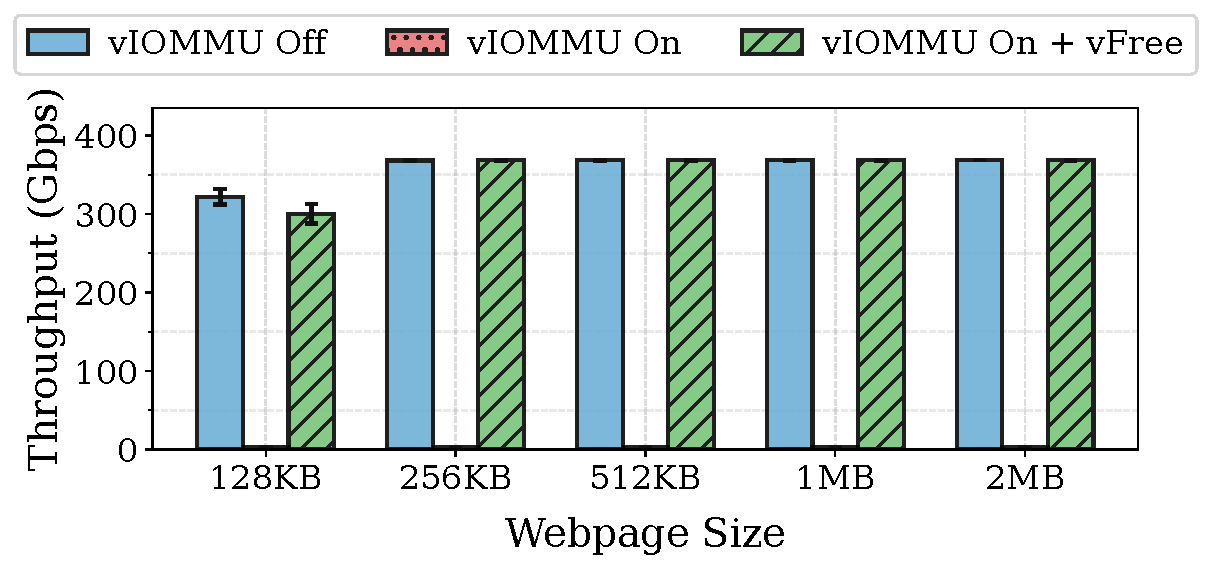
\includegraphics[width=\textwidth]{figures/nginx_size_sweep.pdf}
        \caption{NGINX}
        \label{vfree:fig:nginx}
    \end{subfigure}
    \hfill
    \begin{subfigure}[b]{0.32\textwidth}
        \centering
        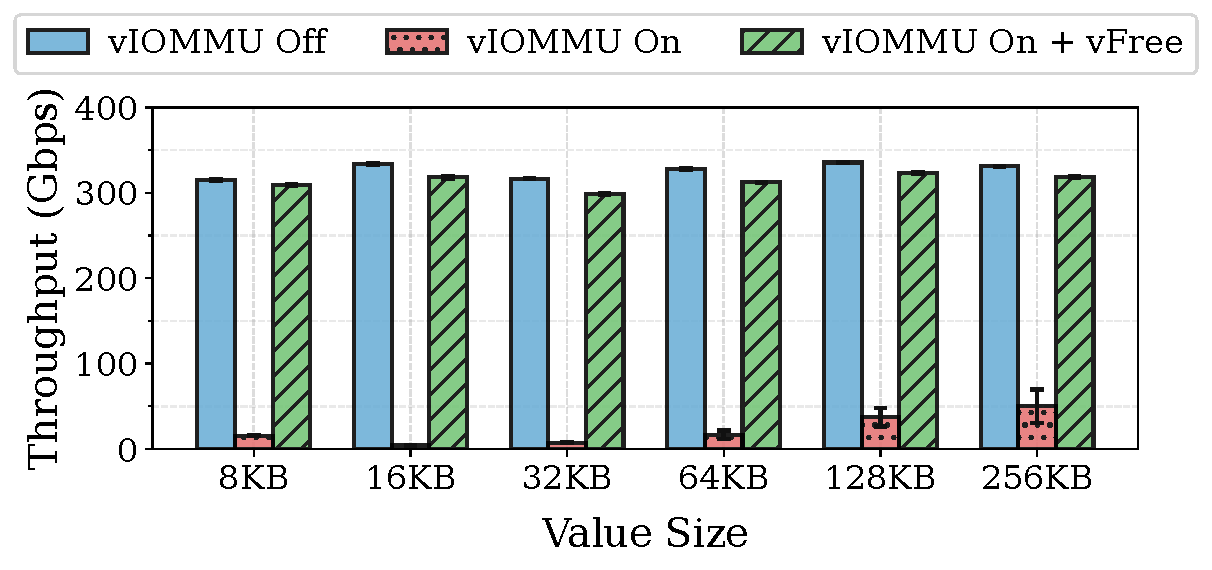
\includegraphics[width=\textwidth]{figures/redis_value_sweep.pdf}
        \caption{Redis}
        \label{vfree:fig:redis}
    \end{subfigure}
    \hfill
    \begin{subfigure}[b]{0.32\textwidth}
        \centering
        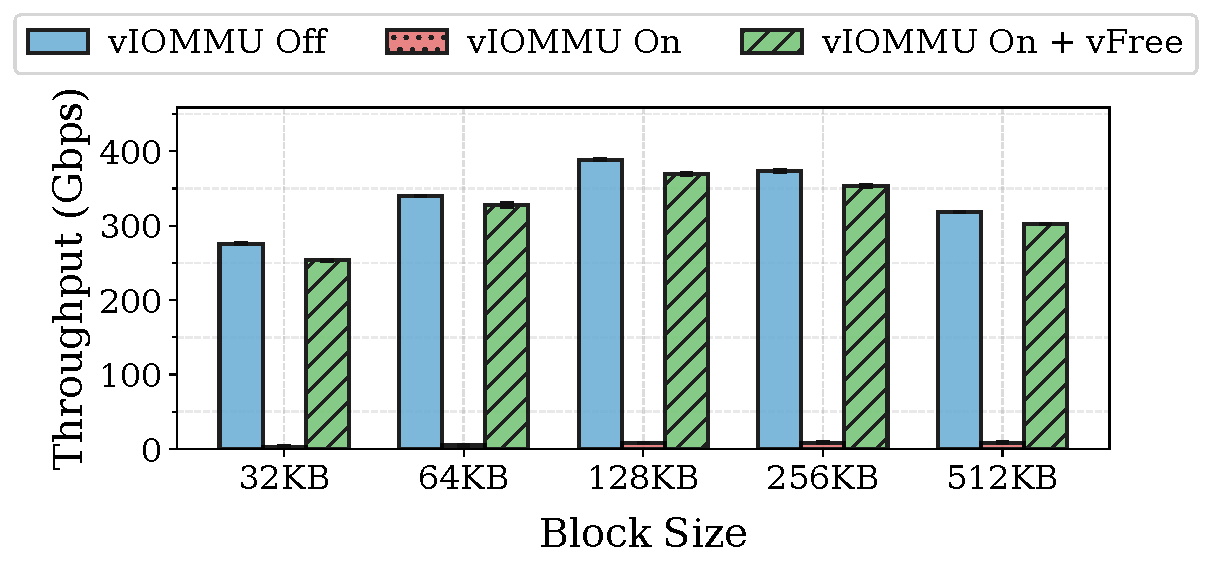
\includegraphics[width=\textwidth]{figures/spdk_fio_block_sizes.pdf}
        \caption{SPDK}
        \label{vfree:fig:spdk}
    \end{subfigure}
    \caption{\small {\bf \vfreebrand enables high-performance networked applications to
        achieve close-to-vIOMMU-off performance with strict protection, 
        consistently delivering low overhead across all evaluated applications.}}
    % Performance of real-world applications across receiver, transmitter, and mixed traffic workloads. 
    % Enabling vIOMMU causes up to 99\% throughput degradation. \vfreebrand delivers close-to-vIOMMU-off performance, with at most an 8\% throughput gap.
    \label{vfree:fig:apps}
\end{figure}


\subsubsection{Code Optimizations}
\label{vfree:sec:other-opt}

% \tianyin{reviewers may ask you how much these optimizations count in your evaluation}

{\bf Reducing critical sections.}
With nested translation,
    invalidation is only required for unmap operations, not map operations~\cite{intel_vtd_spec}.
However, vanilla Linux acquires the per-IO-domain lock at map time
    to check if the domain uses nested translation and if a write-buffer flush is needed for legacy devices.
The implementation is inefficient as both can be determined at domain creation time.
% If neither condition applies, the kernel releases the lock without performing any operation.
% Because the same lock is contended during unmap-side invalidation (\S\ref{vfree:sec:inefficiencies}),
% this unnecessary acquisition at map time exacerbates lock contention.
% We observe that both conditions---first-stage translation mode and write-buffer flush requirement---are
% determined at domain creation time and never change afterward.
\vfreebrand precomputes these attributes and skips the lock acquisition at map time.
% This optimization is general and can be applied to the vanilla kernel as well.

\para{Leveraging IOVA contiguity.}
Inspired by prior work~\cite{Rubin2024FastSafe},
we leverage IOVA contiguity to reduce the number of \CodeIn{map} and \CodeIn{unmap()} calls on the mlx5 Tx path.
Each socket buffer may contain multiple fragments of physically discontinuous pages.
In the vanilla driver, each fragment is mapped and unmapped individually.
We instead use the scatterlist DMA API to map all fragments into a single contiguous IOVA range
and unmap them in a single call, reducing the number of invalidation requests
generated from \CodeIn{unmap()} operations. % (less than 200~LOC).

% Again, the receiver path is optimized with page pool optimization, so the technique is no longer neccessary.



\if 0 % this is too fine-grained
\subsubsection{Runtime Configurability}
Both optimizations are independently controlled via kernel command-line parameters: \texttt{intel\_iommu\_pinned=on|off} selects between the pinned and distributed flush strategies, and
\texttt{intel\_iommu\_dfp=on|off} enables or disables Deferred Page Free.
The maximum number of flush iterations per leader invocation is exposed as a runtime-tunable parameter via \texttt{debugfs}, allowing adjustment without kernel recompilation.
\fi 



